\documentclass[
  final,
  babelLanguage=british,
  %desktopVersion,
  %showtrims,
  %overleaf,
]{anecdote}

%\graphicspath{{./assets/photos/300dpi/}}
\graphicspath{{./assets/photos/92dpi/}}

% Page size: 6x9 inch
% Body text: 10.5 / 15 pt

\usepackage{local}

%% Details of the book
%% ===================

\title{Bhikkhu Manual}
\subtitle{Essential Chants and Vinaya Notes}
\author{Forest Sangha Publications}
\publisher{Forest Sangha Publications}
\date{2019-01-21}
\editionInfo{\textit{Fourth edition}, 2019}
\ISBN{000-000-0000-00-0}% TODO update ISBN

% === Metadata ===

\hypersetup{
  pdftitle={\thetitle},
  pdfauthor={\theauthor},
  pdfcopyright={Copyright (C) 2019, \thePublisher},
  pdfsubject={},% TODO subject
  pdfkeywords={},% TODO keywords
  pdflicenseurl={https://creativecommons.org/licenses/by-nc-nd/4.0/},
  pdfcontacturl={},
  pdflang={en},
}

% FIXME \pdfinfo
%\pdfinfo{%
%  /Title (\thetitle)%
%  /Author (\theauthor)
%  /Subject (subject)% TODO subject
%  /Keywords (keywords)% TODO keywords
%  /GTS_PDFXVersion (PDF/X-1:2001)%
%  /GTS_PDFXConformance (PDF/X-1a:2001)%
%}

%% === Load further packages ===

%% === Hyphenation exceptions and corrections ===

\hyphenation{London}

\begin{document}

\frontmatter

\ifdesktopversion
\desktopCover{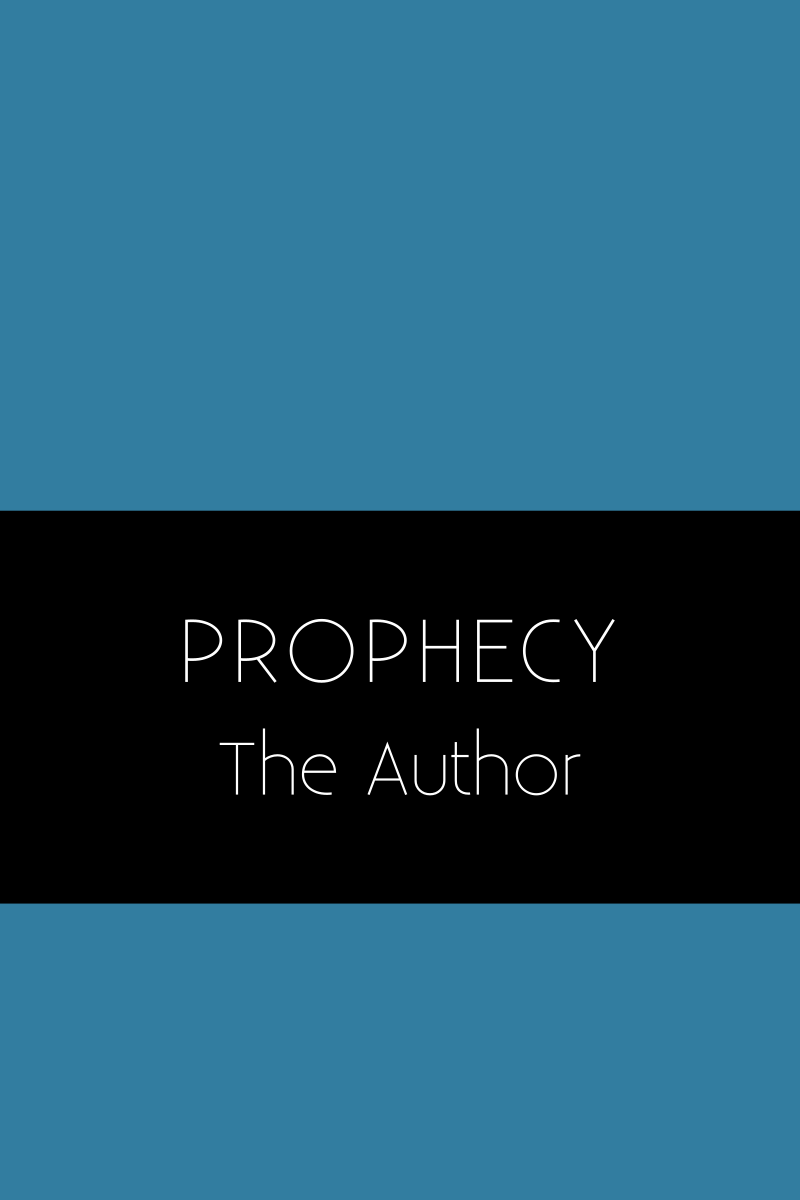
\includegraphics[height=\paperheight]{./desktop-cover.png}}
\fi

\cleartorecto
\thispagestyle{empty}
\vspace*{5em}

{\centering

\settowidth{\titleLength}{%
  {\Large\chapterTitleFont\scshape\MakeLowercase{\thetitle}}%
}

{\Large\chapterTitleFont\thetitle}\\[0.3\baselineskip]
\setlength{\xheight}{\heightof{X}}
\raisebox{0.5\xheight}{\color[gray]{0.4}\rule{\titleLength}{0.25pt}}\\[0.3\baselineskip]
{\itshape
\thesubtitle}

\vfill

\theauthor

\vspace*{5em}

}



\cleartoverso
\thispagestyle{empty}

{\copyrightsize
\centering
\setlength{\parindent}{0pt}%
\setlength{\parskip}{0.8\baselineskip}%

\thetitle\\
\thesubtitle

Published by \thePublisher

ISBN \theISBN

Copyright \copyright\ \thePublisher\ 2020

\vfill

{\footnotesize

This work is licensed under a Creative Commons\\
Attribution-NonCommercial-NoDerivatives 4.0 International~License.

Produced with the \LaTeX\ typesetting system,\\
set in Gentium and Nunito~Sans.

\theEditionInfo

}}


\cleartorecto
\thispagestyle{empty}

\mbox{}\vfill

{\centering\itshape

Namo tassa bhagavato arahato sammāsambuddhassa\\
Namo tassa bhagavato arahato sammāsambuddhassa\\
Namo tassa bhagavato arahato sammāsambuddhassa

}

\vfill\mbox{}

\vspace*{5\baselineskip}



\cleartorecto
\tableofcontents*

%\chapter{Foreword}

Nullam eu ante vel est convallis dignissim. Fusce suscipit, wisi nec facilisis
facilisis, est dui fermentum leo, quis tempor ligula erat quis odio. Nunc porta
vulputate tellus. Nunc rutrum turpis sed pede. Sed bibendum. Aliquam posuere.
Nunc aliquet, augue nec adipiscing interdum, lacus tellus malesuada massa, quis
varius mi purus non odio. Pellentesque condimentum, magna ut suscipit hendrerit,
ipsum augue ornare nulla, non luctus diam neque sit amet urna. Curabitur
vulputate vestibulum lorem. Fusce sagittis, libero non molestie mollis, magna
orci ultrices dolor, at vulputate neque nulla lacinia eros. Sed id ligula quis
est convallis tempor. Curabitur lacinia pulvinar nibh. Nam a sapien.

\bigskip

{\raggedleft
  Reviewer Person\\
  July 2017
\par}


%\chapter{Preface}

Nullam eu ante vel est convallis dignissim. Fusce suscipit, wisi nec facilisis
facilisis, est dui fermentum leo, quis tempor ligula erat quis odio. Nunc porta
vulputate tellus. Nunc rutrum turpis sed pede. Sed bibendum. Aliquam posuere.
Nunc aliquet, augue nec adipiscing interdum, lacus tellus malesuada massa, quis
varius mi purus non odio. Pellentesque condimentum, magna ut suscipit hendrerit,
ipsum augue ornare nulla, non luctus diam neque sit amet urna. Curabitur
vulputate vestibulum lorem. Fusce sagittis, libero non molestie mollis, magna
orci ultrices dolor, at vulputate neque nulla lacinia eros. Sed id ligula quis
est convallis tempor. Curabitur lacinia pulvinar nibh. Nam a sapien.

Nullam eu ante vel est convallis dignissim. Fusce suscipit, wisi nec facilisis
facilisis, est dui fermentum leo, quis tempor ligula erat quis odio. Nunc porta
vulputate tellus. Nunc rutrum turpis sed pede. Sed bibendum. Aliquam posuere.
Nunc aliquet, augue nec adipiscing interdum, lacus tellus malesuada massa, quis
varius mi purus non odio. Pellentesque condimentum, magna ut suscipit hendrerit,
ipsum augue ornare nulla, non luctus diam neque sit amet urna. Curabitur
vulputate vestibulum lorem. Fusce sagittis, libero non molestie mollis, magna
orci ultrices dolor, at vulputate neque nulla lacinia eros. Sed id ligula quis
est convallis tempor. Curabitur lacinia pulvinar nibh. Nam a sapien.

Nullam eu ante vel est convallis dignissim. Fusce suscipit, wisi nec facilisis
facilisis, est dui fermentum leo, quis tempor ligula erat quis odio. Nunc porta
vulputate tellus. Nunc rutrum turpis sed pede. Sed bibendum. Aliquam posuere.
Nunc aliquet, augue nec adipiscing interdum, lacus tellus malesuada massa, quis
varius mi purus non odio. Pellentesque condimentum, magna ut suscipit hendrerit,
ipsum augue ornare nulla, non luctus diam neque sit amet urna. Curabitur
vulputate vestibulum lorem. Fusce sagittis, libero non molestie mollis, magna
orci ultrices dolor, at vulputate neque nulla lacinia eros. Sed id ligula quis
est convallis tempor. Curabitur lacinia pulvinar nibh. Nam a sapien.

\bigskip

{\raggedleft
  The Person\\
  February 2019
\par}



% Page 1 is the first page of the first chapter.
\mainmatter

\chapter{Morning Chanting}

\section{Dedication of Offerings}

[Yo so] bhagavā arahaṃ sammāsambuddho\\
Svākkhāto yena bhagavatā dhammo\\
Supaṭipanno yassa bhagavato sāvakasaṅgho\\
Tam-mayaṃ bhagavantaṃ sadhammaṃ sasaṅghaṃ\\
Imehi sakkārehi yathārahaṃ āropitehi abhipūjayāma\\
Sādhu no bhante bhagavā sucira-parinibbutopi\\
Pacchimā-janatānukampa-mānasā\\
Ime sakkāre duggata-paṇṇākāra-bhūte paṭiggaṇhātu\\
Amhākaṃ dīgharattaṃ hitāya sukhāya\\
Arahaṃ sammāsambuddho bhagavā\\
Buddhaṃ bhagavantaṃ abhivādemi\\\relax
[Svākkhāto] bhagavatā dhammo\\
Dhammaṃ namassāmi\\\relax
[Supaṭipanno] bhagavato sāvakasaṅgho\\
Saṅghaṃ namāmi

\section{Preliminary Homage}

\begin{leader}
  [Handa mayaṃ buddhassa bhagavato pubbabhāga-namakāraṃ karomase]
\end{leader}

Namo tassa bhagavato arahato sammāsambuddhassa

\section{Homage to the Buddha}

\begin{leader}
  [Handa mayaṃ buddhābhitthutiṃ karomase]
\end{leader}

Yo so tathāgato arahaṃ sammāsambuddho\\
Vijjācaraṇa-sampanno\\
Sugato\\
Lokavidū\\
Anuttaro purisadamma-sārathi\\
Satthā deva-manussānaṃ\\
Buddho bhagavā\\
Yo imaṃ lokaṃ sadevakaṃ samārakaṃ sabrahmakaṃ\\
Sassamaṇa-brāhmaṇiṃ pajaṃ sadeva-manussaṃ sayaṃ abhiññā sacchikatvā pavedesi\\
Yo dhammaṃ desesi ādi-kalyāṇaṃ majjhe-kalyāṇaṃ pariyosāna-kalyāṇaṃ\\
Sātthaṃ sabyañjanaṃ kevala-paripuṇṇaṃ parisuddhaṃ brahma-cariyaṃ pakāsesi\\
Tam-ahaṃ bhagavantaṃ abhipūjayāmi tam-ahaṃ bhagavantaṃ sirasā namāmi

\section{Homage to the Dhamma}

\begin{leader}
  [Handa mayaṃ dhammābhitthutiṃ karomase]
\end{leader}

Yo so svākkhāto bhagavatā dhammo\\
Sandiṭṭhiko\\
Akāliko\\
Ehipassiko\\
Opanayiko\\
Paccattaṃ veditabbo viññūhi\\
Tam-ahaṃ dhammaṃ abhipūjayāmi tam-ahaṃ dhammaṃ sirasā namāmi

\section{Homage to the Saṅgha}

\begin{leader}
  [Handa mayaṃ saṅghābhitthutiṃ karomase]
\end{leader}

Yo so supaṭipanno bhagavato sāvakasaṅgho\\
Ujupaṭipanno bhagavato sāvakasaṅgho\\
Ñāyapaṭipanno bhagavato sāvakasaṅgho\\
Sāmīcipaṭipanno bhagavato sāvakasaṅgho\\
Yadidaṃ cattāri purisayugāni aṭṭha purisapuggalā\\
Esa bhagavato sāvakasaṅgho\\
Āhuneyyo\\
Pāhuneyyo\\
Dakkhiṇeyyo\\
Añjali-karaṇīyo\\
Anuttaraṃ puññakkhettaṃ lokassa\\
Tam-ahaṃ saṅghaṃ abhipūjayāmi tam-ahaṃ saṅghaṃ sirasā namāmi

\section{Salutation to the Triple Gem}

TODO


\chapter{Reflection on the Four Requisites}

\begin{leader}
  [Handa mayaṃ taṅkhaṇika-paccavekkhaṇa-pāṭhaṃ bhaṇāmase]
\end{leader}

[Paṭisaṅkhā] yoniso cīvaraṃ paṭisevāmi, yāvadeva sītassa\\
paṭighātāya, uṇhassa paṭighātāya, ḍaṃsa-makasa-vātātapa-siriṃsapa-\\
-samphassānaṃ paṭighātāya, yāvadeva hirikopina-paṭicchādanatthaṃ

[Paṭisaṅkhā] yoniso piṇḍapātaṃ paṭisevāmi, neva davāya, na madāya, na maṇḍanāya, na vibhūsanāya, yāvadeva imassa kāyassa ṭhitiyā, yāpanāya, vihiṃsūparatiyā, brahmacariyānuggahāya, iti purāṇañca vedanaṃ paṭihaṅkhāmi, navañca vedanaṃ na uppādessāmi, yātrā ca me bhavissati anavajjatā ca phāsuvihāro cā'ti

[Paṭisaṅkhā] yoniso senāsanaṃ paṭisevāmi, yāvadeva sītassa\\
paṭighātāya, uṇhassa paṭighātāya, ḍaṃsa-makasa-vātātapa-siriṃsapa-\\
-samphassānaṃ paṭighātāya, yāvadeva utuparissaya vinodanaṃ paṭisallānārāmatthaṃ

[Paṭisaṅkhā] yoniso gilāna-paccaya-bhesajja-parikkhāraṃ paṭisevāmi, yāvadeva uppannānaṃ veyyābādhikānaṃ vedanānaṃ paṭighātāya, abyāpajjha-paramatāyā'ti

\chapter{Five Subjects for Frequent Recollection}

\begin{leader}
  [Handa mayaṃ abhiṇha-paccavekkhaṇa-pāṭhaṃ bhaṇāmase]
\end{leader}

\sidepar{Men Chant}%
[Jarā-dhammomhi] jaraṃ anatīto

\sidepar{Women Chant}%
[Jarā-dhammāmhi] jaraṃ anatītā

\sidepar{m.}%
Byādhi-dhammomhi byādhiṃ anatīto

\sidepar{w.}%
Byādhi-dhammāmhi byādhiṃ anatītā

\sidepar{m.}%
Maraṇa-dhammomhi maraṇaṃ anatīto

\sidepar{w.}%
Maraṇa-dhammāmhi maraṇaṃ anatītā

Sabbehi me piyehi manāpehi nānābhāvo vinābhāvo

\sidepar{m.}%
Kammassakomhi kammadāyādo kammayoni kammabandhu kammapaṭisaraṇo\\
Yaṃ kammaṃ karissāmi, kalyāṇaṃ vā pāpakaṃ vā, tassa dāyādo bhavissāmi

\sidepar{w.}%
Kammassakāmhi kammadāyādā kammayoni kammabandhu kammapaṭisaraṇā\\
Yaṃ kammaṃ karissāmi, kalyāṇaṃ vā pāpakaṃ vā, tassa dāyādā bhavissāmi

Evaṃ amhehi abhiṇhaṃ paccavekkhitabbaṃ

\chapter{Patti-dāna-gāthā}

\begin{leader}
  [Handa mayaṃ patti-dāna-gāthāyo bhaṇāmase.]
\end{leader}

Yā devatā santi vihāra-vāsinī\\
Thūpe ghare bodhi-ghare tahiṃ tahiṃ\\
Tā dhamma-dānena bhavantu pūjitā\\
Sotthiṃ karonte’dha vihāra-maṇḍale\\
Therā ca majjhā navakā ca bhikkhavo\\
Sārāmikā dāna-patī upāsakā\\
Gāmā ca desā nigamā ca issarā\\
Sappāṇa-bhūtā sukhitā bhavantu te\\
Jalābu-jā ye pi ca aṇḍa-sambhavā\\
Saṃseda-jātā atha-v-opapātikā\\
Niyyānikaṃ dhamma-varaṃ paṭicca te\\
Sabbe pi dukkhassa karontu saṅkhayaṃ.\\
Ṭhātu ciraṃ sataṃ dhammo\\
Dhamma-dharā ca puggalā\\
Saṅgho hotu samaggo va\\
Atthāya ca hitāya ca\\
Amhe rakkhatu saddhammo\\
Sabbe pi dhamma-cārino\\
Vuḍḍhiṃ sampāpuṇeyyāma\\
Dhamme ariyappavedite.

(♦) Pasannā hontu sabbe pi\\
Pāṇino Buddha-sāsane.\\
Sammā-dhāraṃ pavecchanto\\
Kāle devo pavassatu.\\
Vuḍḍhi-bhāvāya sattānaṃ\\
Samiddhaṃ netu medaniṃ.\\
Mātā-pitā ca atra-jaṃ\\
Niccaṃ rakkhanti puttakaṃ.\\
Evaṃ dhammena rājāno\\
Pajaṃ rakkhantu sabbadā.


\chapter{Evening Chanting}

\chapter*{Dedication of Offerings}

[Yo so] bhagavā arahaṃ sammāsambuddho\\
Svākkhāto yena bhagavatā dhammo\\
Supaṭipanno yassa bhagavato sāvakasaṅgho\\
Tam-mayaṃ bhagavantaṃ sadhammaṃ sasaṅghaṃ\\
Imehi sakkārehi yathārahaṃ āropitehi abhipūjayāma\\
Sādhu no bhante bhagavā sucira-parinibbutopi\\
Pacchimā-janatānukampa-mānasā\\
Ime sakkāre duggata-paṇṇākāra-bhūte paṭiggaṇhātu\\
Amhākaṃ dīgharattaṃ hitāya sukhāya\\
Arahaṃ sammāsambuddho bhagavā\\
Buddhaṃ bhagavantaṃ abhivādemi \instr{Bow}

[Svākkhāto] bhagavatā dhammo\\
Dhammaṃ namassāmi \instr{Bow}

[Supaṭipanno] bhagavato sāvakasaṅgho\\
Saṅghaṃ namāmi \instr{Bow}

(NOTE: additional chanting)

[Yam-amha kho mayaṃ Bhagavantaṃ saraṇaṃ
gatā, uddissa pabbajitā yo no Bhagavā satthā,
yassa ca mayaṃ Bhagavato dhammaṃ rocema.
Imehi sakkārehi taṃ Bhagavantaṃ sasaddhammaṃ sasāvaka-saṅghaṃ abhipūjayāma.]

\chapter*{Preliminary Homage}

\begin{leader}
  [Handa mayaṃ buddhassa bhagavato pubbabhāga-namakāraṃ karomase]
\end{leader}

Namo tassa bhagavato arahato sammāsambuddhassa

\instr{Three times}

\chapter*{Recollection of the Buddha}

\begin{leader}
  [Handa mayaṃ buddhānussatinayaṃ karomase]
\end{leader}

Taṃ kho pana bhagavantaṃ evaṃ kalyāṇo kittisaddo abbhuggato\\
Itipi so bhagavā arahaṃ sammāsambuddho\\
Vijjācaraṇa-sampanno sugato lokavidū\\
Anuttaro purisadamma-sārathi satthā deva-manussānaṃ\\
\vin buddho bhagavā'ti

\chapter*{Supreme Praise of the Buddha}

\begin{leader}
  [Handa mayaṃ buddhābhigītiṃ karomase]
\end{leader}

Buddh'vārahanta-varatādiguṇābhiyutto\\
Suddhābhiñāṇa-karuṇāhi samāgatatto\\
Bodhesi yo sujanataṃ kamalaṃ va sūro\\
Vandām'ahaṃ tam-araṇaṃ sirasā jinendaṃ\\
Buddho yo sabba-pāṇīnaṃ saraṇaṃ khemam-uttamaṃ\\
Paṭhamānussatiṭṭhānaṃ vandāmi taṃ siren'ahaṃ\\
Buddhassāh'asmi dāso/dāsī va buddho me sāmi-kissaro\\
Buddho dukkhassa ghātā ca vidhātā ca hitassa me\\
Buddhass'āhaṃ niyyādemi sarīrañ-jīvitañ-cidaṃ\\
Vandanto'haṃ/Vandantī'haṃ carissāmi buddhass'eva subodhitaṃ\\
Natthi me saraṇaṃ aññaṃ buddho me saraṇaṃ varaṃ\\
Etena sacca-vajjena vaḍḍheyyaṃ satthu-sāsane\\
Buddhaṃ me vandamānena/vandamānāya\\
\vin yaṃ puññaṃ pasutaṃ idha\\
Sabbepi antarāyā me māhesuṃ tassa tejasā

\begin{instruction}
  Bowing
\end{instruction}

Kāyena vācāya va cetasā vā\\
Buddhe kukammaṃ pakataṃ mayā yaṃ\\
Buddho paṭiggaṇhātu accayantaṃ\\
Kālantare saṃvarituṃ va buddhe

\chapter*{Recollection of the Dhamma}

\begin{leader}
  [Handa mayaṃ dhammānussatinayaṃ karomase]
\end{leader}

Svākkhāto bhagavatā dhammo\\
Sandiṭṭhiko akāliko ehipassiko\\
Opanayiko paccattaṃ veditabbo viññūhī'ti

\chapter*{Supreme Praise of the Dhamma}

\begin{leader}
  [Handa mayaṃ dhammābhigītiṃ karomase]
\end{leader}

Svākkhātat'ādiguṇa-yoga-vasena seyyo\\
Yo magga-pāka-pariyatti-vimokkha-bhedo\\
Dhammo kuloka-patanā tada-dhāri-dhārī\\
Vandām'ahaṃ tama-haraṃ vara-dhammam-etaṃ\\
Dhammo yo sabba-pāṇīnaṃ saraṇaṃ khemam-uttamaṃ\\
Dutiyānussatiṭṭhānaṃ vandāmi taṃ siren'ahaṃ\\
Dhammassāh'asmi dāso/dāsī va dhammo me sāmi-kissaro\\
Dhammo dukkhassa ghātā ca vidhātā ca hitassa me\\
Dhammass'āhaṃ niyyādemi sarīrañ-jīvitañ-cidaṃ\\
Vandantohaṃ/Vandantīhaṃ carissāmi dhammass'eva sudhammataṃ\\
Natthi me saraṇaṃ aññaṃ dhammo me saraṇaṃ varaṃ\\
Etena sacca-vajjena vaḍḍheyyaṃ satthu-sāsane\\
Dhammaṃ me vandamānena/vandamānāya\\
\vin yaṃ puññaṃ pasutaṃ idha\\
Sabbepi antarāyā me māhesuṃ tassa tejasā

\begin{instruction}
  Bowing
\end{instruction}

Kāyena vācāya va cetasā vā\\
Dhamme kukammaṃ pakataṃ mayā yaṃ\\
Dhammo paṭiggaṇhātu accayantaṃ\\
Kālantare saṃvarituṃ va dhamme

\chapter*{Recollection of the Saṅgha}

\begin{leader}
  [Handa mayaṃ saṅghānussatinayaṃ karomase]
\end{leader}

Supaṭipanno bhagavato sāvakasaṅgho\\
Ujupaṭipanno bhagavato sāvakasaṅgho\\
Ñāyapaṭipanno bhagavato sāvakasaṅgho\\
Sāmīcipaṭipanno bhagavato sāvakasaṅgho\\
Yadidaṃ cattāri purisayugāni aṭṭha purisapuggalā\\
Esa bhagavato sāvakasaṅgho\\
Āhuneyyo pāhuneyyo dakkhiṇeyyo añjali-karaṇīyo\\
Anuttaraṃ puññakkhettaṃ lokassā'ti

\chapter*{Supreme Praise of the Saṅgha}

\begin{leader}
  [Handa mayaṃ saṅghābhigītiṃ karomase]
\end{leader}

Saddhammajo supaṭipatti-guṇādiyutto\\
Yo'ṭṭhabbidho ariyapuggala-saṅgha-seṭṭho\\
Sīlādidhamma-pavarāsaya-kāya-citto\\
Vandām'ahaṃ tam-ariyāna-gaṇaṃ susuddhaṃ\\
Saṅgho yo sabba-pāṇīnaṃ saraṇaṃ khemam-uttamaṃ\\
Tatiyānussatiṭṭhānaṃ vandāmi taṃ siren'ahaṃ

Saṅghass'āhasmi dāso/dāsī va saṅgho me sāmi-kissaro\\
Saṅgho dukkhassa ghātā ca vidhātā ca hitassa me\\
Saṅghass'āhaṃ niyyādemi sarīrañ-jīvitañ-cidaṃ\\
Vandanto'haṃ/Vandantī'haṃ carissāmi saṅghassopaṭipannataṃ\\
Natthi me saraṇaṃ aññaṃ saṅgho me saraṇaṃ varaṃ\\
Etena sacca-vajjena vaḍḍheyyaṃ satthu-sāsane\\
Saṅghaṃ me vandamānena/vandamānāya\\
\vin yaṃ puññaṃ pasutaṃ idha\\
Sabbepi antarāyā me māhesuṃ tassa tejasā

\begin{instruction}
  Bowing
\end{instruction}

Kāyena vācāya va cetasā vā\\
Saṅghe kukammaṃ pakataṃ mayā yaṃ\\
Saṅgho paṭiggaṇhātu accayantaṃ\\
Kālantare saṃvarituṃ va saṅghe

\chapter*{Closing Homage}

[Arahaṃ] sammāsambuddho bhagavā\\
Buddhaṃ bhagavantaṃ abhivādemi \instr{Bow}

[Svākkhāto] bhagavatā dhammo\\
Dhammaṃ namassāmi \instr{Bow}

[Supaṭipanno] bhagavato sāvakasaṅgho\\
Saṅghaṃ namāmi \instr{Bow}


\chapter{Paritta Chants}

\chapter{Requesting Paritta Chanting}

\begin{instruction}
  After bowing three times, with hands joined in añjali,\\
  recite the following
\end{instruction}

Vipatti-paṭibāhāya sabba-sampatti-siddhiyā\\
Sabbadukkha-vināsāya\\
Parittaṃ brūtha maṅgalaṃ

Vipatti-paṭibāhāya sabba-sampatti-siddhiyā\\
Sabbabhaya-vināsāya\\
Parittaṃ brūtha maṅgalaṃ

Vipatti-paṭibāhāya sabba-sampatti-siddhiyā\\
Sabbaroga-vināsāya\\
Parittaṃ brūtha maṅgalaṃ

\begin{instruction}
  Bow three times
\end{instruction}

\chapter{Invitation to the Devas}

(NOTE: is this an alternative beginning?)

Sarajjaṃ sasenaṃ sabandhuṃ nar’indaṃ,\\
Paritt’ānubhavo sadā rakkhatū-ti,

\begin{paritta}
\sidepar{A.}%
Pharitvāna mettaṃ samettā bhadantā\\
Avikkhitta-cittā parittaṃ bhaṇantu

\sidepar{B.}%
Samantā cakka-vāḷesu\\
Atr'āgacchantu devatā

Sagge kāme ca rūpe\\
Giri-sikhara-taṭe c'antalikkhe vimāne\\
Dīpe raṭṭhe ca gāme\\
Taru-vana-gahane geha-vatthumhi khette\\
Bhummā c'āyantu devā\\
Jala-thala-visame yakkha-gandhabba-nāgā\\
Tiṭṭhantā santike yaṃ\\
Muni-vara-vacanaṃ sādhavo me suṇantu

Dhammassavana-kālo ayam-bhadantā

\instr{Three times, or}

Buddha-dassana-kālo ayam-bhadantā\\
Dhammassavana-kālo ayam-bhadantā\\
Saṅgha-payirūpāsana-kālo ayam-bhadantā
\end{paritta}

\chapter{Pubba-bhāga-nama-kāra-pāṭho}

\begin{paritta}
Namo tassa bhagavato arahato sammā-sambuddhassa\\
Namo tassa bhagavato arahato sammā-sambuddhassa\\
Namo tassa bhagavato arahato sammā-sambuddhassa
\end{paritta}

\chapter{Saraṇa-gamana-pāṭho}

\begin{paritta}
Buddhaṃ saraṇaṃ gacchāmi\\
Dhammaṃ saraṇaṃ gacchāmi\\
Saṅghaṃ saraṇaṃ gacchāmi

Dutiyam pi buddhaṃ saraṇaṃ gacchāmi\\
Dutiyam pi dhammaṃ saraṇaṃ gacchāmi\\
Dutiyam pi saṅghaṃ saraṇaṃ gacchāmi

Tatiyam pi buddhaṃ saraṇaṃ gacchāmi\\
Tatiyam pi dhammaṃ saraṇaṃ gacchāmi\\
Tatiyam pi saṅghaṃ saraṇaṃ gacchāmi
\end{paritta}

\chapter{Nama-kāra-siddhi-gāthā}

\begin{paritta}
Yo cakkhumā moha-malāpakaṭṭho\\
Sāmaṃ va buddho sugato vimutto\\
Mārassa pāsā vinimocayanto\\
Pāpesi khemaṃ janataṃ vineyyaṃ\\
Buddhaṃ varan-taṃ sirasā namāmi\\
Lokassa nāthañ-ca vināyakañ-ca\\
Tan-tejasā te jaya-siddhi hotu\\
Sabb'antarāyā ca vināsamentu

Dhammo dhajo yo viya tassa satthu\\
Dassesi lokassa visuddhi-maggaṃ\\
Niyyāniko dhamma-dharassa dhārī\\
Sāt'āvaho santi-karo suciṇṇo\\
Dhammaṃ varan-taṃ sirasā namāmi\\
Mohappadālaṃ upasanta-dāhaṃ\\
Tan-tejasā te jaya-siddhi hotu\\
Sabb'antarāyā ca vināsamentu

Saddhamma-senā sugatānugo yo\\
Lokassa pāpūpakilesa-jetā\\
Santo sayaṃ santi-niyojako ca\\
Svākkhāta-dhammaṃ viditaṃ karoti\\
Saṅghaṃ varan-taṃ sirasā namāmi\\
Buddhānubuddhaṃ sama-sīla-diṭṭhiṃ\\
Tan-tejasā te jaya-siddhi hotu\\
Sabb'antarāyā ca vināsamentu
\end{paritta}

\chapter{Sacca-kiriyā-gāthā}

Natthi me saraṇaṃ aññaṃ buddho me saraṇaṃ varaṃ\\
Etena sacca-vajjena sotthi te/me hotu sabbadā

Natthi me saraṇaṃ aññaṃ dhammo me saraṇaṃ varaṃ\\
Etena sacca-vajjena sotthi te/me hotu sabbadā

Natthi me saraṇaṃ aññaṃ saṅgho me saraṇaṃ varaṃ\\
Etena sacca-vajjena sotthi te/me hotu sabbadā

\chapter{Mahā-kāruṇiko nātho ti ādikā gāthā}

Mahā-kāruṇiko nātho\\
Atthāya sabba-pāṇinaṃ\\
Hitāya sabba-pāṇinaṃ\\
Sukhāya sabba-pāṇinaṃ

Pūretvā pāramī sabbā\\
Patto sambodhim-uttamaṃ\\
Etena sacca-vajjena\\
Mā hontu sabb'upaddavā.

\chapter{Namo-kāra-aṭṭhaka}

\begin{paritta}
Namo arahato sammā\\
Sambuddhassa mahesino\\
Namo uttama-dhammassa\\
Svākkhātass'eva ten'idha\\
Namo mahā-saṅghassāpi\\
Visuddha-sīla-diṭṭhino\\
Namo omāty-āraddhassa\\
Ratanattayassa sādhukaṃ\\
Namo omakātītassa\\
Tassa vatthuttayassa-pi\\
Namo-kārappabhāvena\\
Vigacchantu upaddavā\\
Namo-kārānubhāvena\\
Suvatthi hotu sabbadā\\
Namo-kārassa tejena\\
Vidhimhi homi tejavā\\
\end{paritta}

\chapter{Maṅgala-sutta}

(NOTE: additional intro)

Evam-me sutaṃ: Ekaṃ samayaṃ Bhagavā,
Sāvatthiyaṃ viharati, Jeta-vane Anāthapiṇḍikassa ārāme.
Atha kho aññatarā devatā abhikkantāya
rattiyā abhikkanta-vaṇṇā kevala-kappaṃ Jetavanaṃ obhāsetvā, yena Bhagavā ten’upasaṅkami. Upasaṅkamitvā Bhagavantaṃ
abhivādetvā ekam-antaṃ aṭṭhāsi. Ekam-antaṃ
ṭhitā kho sā devatā Bhagavantaṃ gāthāya
ajjhabhāsi:
Bahū devā manussā ca,
Maṅgalāni acintayuṃ;
Ākaṅkhamānā sotthānaṃ,
Brūhi maṅgalam-uttamaṃ.

\begin{paritta}
Asevanā ca bālānaṃ\\
Paṇḍitānañ-ca sevanā\\
Pūjā ca pūjanīyānaṃ\\
Etam maṅgalam-uttamaṃ

Paṭirūpa-desa-vāso ca\\
Pubbe ca kata-puññatā\\
Atta-sammā-paṇidhi ca\\
Etam maṅgalam-uttamaṃ

Bāhu-saccañ-ca sippañ-ca,\\
Vinayo ca susikkhito\\
Subhāsitā ca yā vācā\\
Etam maṅgalam-uttamaṃ

Mātā-pitu-upaṭṭhānaṃ\\
Putta-dārassa saṅgaho\\
Anākulā ca kammantā\\
Etam maṅgalam-uttamaṃ

Dānañ-ca dhamma-cariyā ca\\
Ñātakānañ-ca saṅgaho\\
Anavajjāni kammāni\\
Etam maṅgalam-uttamaṃ

Āratī viratī pāpā\\
Majja-pānā ca saññamo\\
Appamādo ca dhammesu\\
Etam maṅgalam-uttamaṃ

Gāravo ca nivāto ca\\
Santuṭṭhī ca kataññutā\\
Kālena dhammassavanaṃ\\
Etam maṅgalam-uttamaṃ

Khantī ca sovacassatā\\
Samaṇānañ-ca dassanaṃ\\
Kālena dhamma-sākacchā\\
Etam maṅgalam-uttamaṃ

Tapo ca brahma-cariyañ-ca\\
Ariya-saccāna-dassanaṃ\\
Nibbāna-sacchikiriyā ca\\
Etam maṅgalam-uttamaṃ

Phuṭṭhassa loka-dhammehi\\
Cittaṃ yassa na kampati\\
Asokaṃ virajaṃ khemaṃ\\
Etam maṅgalam-uttamaṃ

Etādisāni katvāna\\
Sabbattham-aparājitā\\
Sabbattha sotthiṃ gacchanti\\
Tan-tesaṃ maṅgalam-uttaman'ti

\end{paritta}

\chapter{Ratana Sutta}

(NOTE: alternative beginning)

Yānīdha bhūtāni samāgatāni,\\
Bhummāni vā yāni va antalikkhe.\\
Sabb’eva bhūtā sumanā bhavantu,\\
Atho pi sakkacca suṇantu bhāsitaṃ.\\
Tasmā hi bhūtā nisāmetha sabbe,\\
Mettaṃ karotha mānusiyā pajāya.\\
Divā ca ratto ca haranti ye baliṃ,\\
Tasmā hi ne rakkhatha appamattā.

(♦1) Yaṅkiñci vittaṃ idha vā huraṃ vā\\
Saggesu vā yaṃ ratanaṃ paṇītaṃ\\
Na no samaṃ atthi tathāgatena\\
Idam-pi buddhe ratanaṃ paṇītaṃ\\
Etena saccena suvatthi hotu

(♦2) Khayaṃ virāgaṃ amataṃ paṇītaṃ\\
Yad-ajjhagā sakya-munī samāhito\\
Na tena dhammena sam'atthi kiñci\\
Idam-pi dhamme ratanaṃ paṇītaṃ\\
Etena saccena suvatthi hotu

(♦3) Yam buddha-seṭṭho parivaṇṇayī suciṃ\\
Samādhim-ānantarikaññam-āhu\\
Samādhinā tena samo na vijjati\\
Idam-pi dhamme ratanaṃ paṇītaṃ\\
Etena saccena suvatthi hotu

(♦4) Ye puggalā aṭṭha sataṃ pasaṭṭhā\\
Cattāri etāni yugāni honti\\
Te dakkhiṇeyyā sugatassa sāvakā\\
Etesu dinnāni mahapphalāni\\
Idam-pi saṅghe ratanaṃ paṇītaṃ\\
Etena saccena suvatthi hotu

(♦5) Ye suppayuttā manasā daḷhena\\
Nikkāmino gotama-sāsanamhi\\
Te patti-pattā amataṃ vigayha\\
Laddhā mudhā nibbutiṃ bhuñjamānā\\
Idam-pi saṅghe ratanaṃ paṇītaṃ\\
Etena saccena suvatthi hotu

Yath’inda-khīlo paṭhaviṃ sito siyā,\\
Catubbhi vātebhi asampakampiyo.\\
Tathūpamaṃ sappurisaṃ vadāmi,\\
Yo ariya-saccāni avecca passati.\\
Idam-pi Saṅghe ratanaṃ paṇītaṃ,\\
Etena saccena suvatthi hotu.

Ye ariya-saccāni vibhāvayanti,\\
Gambhīra-paññena sudesitāni.\\
Kiñ-cāpi te honti bhusappamattā,\\
Na te bhavaṃ aṭṭhamam-ādiyanti.\\
Idam-pi Saṅghe ratanaṃ paṇītaṃ,\\
Etena saccena suvatthi hotu.

Sahā v’assa dassana-sampadāya,\\
Tay’assu dhammā jahitā bhavanti.\\
Sakkāya-diṭṭhi vicikicchitañ-ca,\\
Sīlabbataṃ vā pi yad-atthi kiñci.\\
Catūh’apāyehi ca vippamutto,\\
Cha cābhiṭhānāni abhabbo kātuṃ.\\
Idam-pi Saṅghe ratanaṃ paṇītaṃ,\\
Etena saccena suvatthi hotu.

Kiñ-cāpi so kammaṃ karoti pāpakaṃ,\\
Kāyena vācā uda cetasā vā.\\
Abhabbo so tassa paṭicchadāya,\\
Abhabbatā diṭṭha-padassa vuttā.\\
Idam-pi Saṅghe ratanaṃ paṇītaṃ,\\
Etena saccena suvatthi hotu.

Vanappagumbe yathā phussi-t-agge,\\
Gimhāna-māse paṭhamasmiṃ gimhe.\\
Tathūpamaṃ dhamma-varaṃ adesayi,\\
Nibbāna-gāmiṃ paramaṃ hitāya.\\
Idam-pi Buddhe ratanaṃ paṇītaṃ,\\
Etena saccena suvatthi hotu.

Varo varañ-ñū vara-do var’āharo,\\
Anuttaro dhamma-varaṃ adesayi.\\
Idam-pi Buddhe ratanaṃ paṇītaṃ,\\
Etena saccena suvatthi hotu.

(♦6) Khīṇaṃ purāṇaṃ navaṃ n'atthi sambhavaṃ\\
Viratta-citt'āyatike bhavasmiṃ\\
Te khīṇa-bījā aviruḷhi-chandā\\
Nibbanti dhīrā yathā'yam padīpo\\
Idam-pi saṅghe ratanaṃ paṇītaṃ\\
Etena saccena suvatthi hotu

Yānīdha bhūtāni samāgatāni,\\
Bhummāni vā yāni va antalikkhe.\\
Tathāgataṃ deva-manussa-pūjitaṃ,\\
Buddhaṃ namassāma suvatthi hotu.

Yānīdha bhūtāni samāgatāni,\\
Bhummāni vā yāni va antalikkhe.\\
Tathāgataṃ deva-manussa-pūjitaṃ,\\
Dhammaṃ namassāma suvatthi hotu.

Yānīdha bhūtāni samāgatāni,\\
Bhummāni vā yāni va antalikkhe.\\
Tathāgataṃ deva-manussa-pūjitaṃ,\\
Saṅghaṃ namassāma suvatthi hotū-ti.

\chapter{Karaṇīya-metta-sutta}

\begin{paritta}
Karaṇīyam-attha-kusalena\\
Yan-taṃ santaṃ padaṃ abhisamecca\\
Sakko ujū ca suhujū ca\\
Suvaco c'assa mudu anatimānī

Santussako ca subharo ca\\
Appakicco ca sallahuka-vutti\\
Sant'indriyo ca nipako ca\\
Appagabbho kulesu ananugiddho

Na ca khuddaṃ samācare kiñci\\
Yena viññū pare upavadeyyuṃ\\
Sukhino vā khemino hontu\\
Sabbe sattā bhavantu sukhit'attā

Ye keci pāṇa-bhūt'atthi\\
Tasā vā thāvarā vā anavasesā\\
Dīghā vā ye mahantā vā\\
Majjhimā rassakā aṇuka-thūlā

Diṭṭhā vā ye ca adiṭṭhā\\
Ye ca dūre vasanti avidūre\\
Bhūtā vā sambhavesī vā\\
Sabbe sattā bhavantu sukhit'attā

Na paro paraṃ nikubbetha\\
Nātimaññetha katthaci naṃ kiñci\\
Byārosanā paṭighasaññā\\
Nāññam-aññassa dukkham-iccheyya

Mātā yathā niyaṃ puttaṃ\\
Āyusā eka-puttam-anurakkhe\\
Evam'pi sabba-bhūtesu\\
Mānasam-bhāvaye aparimāṇaṃ

Mettañ-ca sabba-lokasmiṃ\\
Mānasam-bhāvaye aparimāṇaṃ\\
Uddhaṃ adho ca tiriyañ-ca\\
Asambādhaṃ averaṃ asapattaṃ

Tiṭṭhañ-caraṃ nisinno vā\\
Sayāno vā yāvat'assa vigata-middho\\
Etaṃ satiṃ adhiṭṭheyya\\
Brahmam-etaṃ vihāraṃ idham-āhu

Diṭṭhiñca anupagamma\\
Sīlavā dassanena sampanno\\
Kāmesu vineyya gedhaṃ\\
Na hi jātu gabbha-seyyaṃ punaretī'ti
\end{paritta}

\chapter{Khandha-parittaṃ}

\begin{twochants}
Virūpakkhehi me mettaṃ & mettaṃ erāpathehi me\\
Chabyā-puttehi me mettaṃ & mettaṃ kaṇhā-gotamakehi ca\\
Apādakehi me mettaṃ & mettaṃ dipādakehi me\\
Catuppadehi me mettaṃ & mettaṃ bahuppadehi me\\
Mā maṃ apādako hiṃsi & mā maṃ hiṃsi dipādako\\
Mā maṃ catuppado hiṃsi & mā maṃ hiṃsi bahuppado\\
Sabbe sattā sabbe pāṇā & sabbe bhūtā ca kevalā\\
Sabbe bhadrāni passantu & mā kiñci pāpam-āgamā\\
Appamāṇo buddho & appamāṇo dhammo\\
Appamāṇo saṅgho & pamāṇavantāni siriṃsapāni\\
Ahi-vicchikā sata-padī & uṇṇā-nābhī sarabhū mūsikā\\
Katā me rakkhā katā me parittā & paṭikkamantu bhūtāni\\
So'haṃ namo bhagavato & namo sattannaṃ\\
Sammā-sambuddhānaṃ & \\
\end{twochants}

\chapter{Mora-parittaṃ}

% TODO complete and format

Udet’ayañ-cakkhumā eka-rājā, [ a.m.]\\
Apet’ayañ-cakkhumā eka-rājā, [ p.m.]

...

\chapter{Vaṭṭaka-parittaṃ}

\begin{twochants}
Atthi loke sīla-guṇo & saccaṃ soceyy'anuddayā\\
Tena saccena kāhāmi & sacca-kiriyam-anuttaraṃ\\
Āvajjitvā dhamma-balaṃ & saritvā pubbake jine\\
Sacca-balam-avassāya & sacca-kiriyam-akās'ahaṃ\\
Santi pakkhā apattanā & santi pādā avañcanā\\
Mātā pitā ca nikkhantā & jāta-veda paṭikkama\\
Saha sacce kate mayhaṃ & mahā-pajjalito sikhī\\
Vajjesi soḷasa karīsāni & udakaṃ patvā yathā sikhī\\
Saccena me samo n'atthi & esā me sacca-pāramī ti\\
\end{twochants}

\chapter{Buddha-dhamma-saṅgha-guṇā}

\begin{paritta}

Iti pi so bhagavā arahaṃ sammā-sambuddho\\
Vijjā-caraṇa-sampanno sugato loka-vidū\\
Anuttaro purisa-damma-sārathi\\
Satthā devamanussānaṃ buddho bhagavā'ti

Svākkhāto bhagavatā dhammo sandiṭṭhiko akāliko ehi-passiko\\
Opanayiko paccattaṃ veditabbo viññūhī'ti

Supaṭipanno bhagavato sāvaka-saṅgho\\
Uju-paṭipanno bhagavato sāvaka-saṅgho\\
Ñāya-paṭipanno bhagavato sāvaka-saṅgho\\
Sāmīci-paṭipanno bhagavato sāvaka-saṅgho\\
Yad-idaṃ cattāri purisa-yugāni aṭṭha purisa-puggalā\\
Esa bhagavato sāvaka-saṅgho\\
Āhuneyyo pāhuneyyo dakkhiṇeyyo añjali-karaṇīyo\\
Anuttaraṃ puññakkhettaṃ lokassā'ti

(♦) Araññe rukkha-mūle vā\\
Suññāgāre va bhikkhavo\\
Anussaretha Sambuddhaṃ\\
Bhayaṃ tumhāka no siyā.\\
No ce Buddhaṃ sareyyātha\\
Loka-jeṭṭhaṃ nar’āsabhaṃ\\
Atha dhammaṃ sareyyātha\\
Niyyānikaṃ sudesitaṃ.\\
No ce dhammaṃ sareyyātha\\
Niyyānikaṃ sudesitaṃ\\
Atha saṅghaṃ sareyyātha\\
Puññakkhettaṃ anuttaraṃ.\\
Evam-Buddhaṃ sarantānaṃ\\
Dhammaṃ saṅghañ-ca bhikkhavo\\
Bhayaṃ vā chambhitattaṃ vā\\
Loma-haṃso na hessatī-ti.

\end{paritta}

\chapter{Āṭānāṭiya Paritta (short)}

\begin{twochants}
Vipassissa nam'atthu & cakkhumantassa sirīmato\\
Sikhissa pi nam'atthu & sabba-bhūtānukampino\\
Vessabhussa nam'atthu & nhātakassa tapassino\\
Nam'atthu kakusandhassa & māra-senappamaddino\\
Konāgamanassa nam'atthu & brāhmaṇassa vusīmato\\
Kassapassa nam'atthu & vippamuttassa sabbadhi\\
Aṅgīrasassa nam'atthu & sakya-puttassa sirīmato\\
Yo imaṃ dhammam-adesesi & sabba-dukkhāpanūdanaṃ\\
Ye cāpi nibbutā loke & yathā-bhūtaṃ vipassisuṃ\\
Te janā apisuṇā & mahantā vīta-sāradā\\
Hitaṃ deva-manussānaṃ & yaṃ namassanti gotamaṃ\\
Vijjā-caraṇa-sampannaṃ & mahantaṃ vīta-sāradaṃ\\
Vijjā-caraṇa-sampannaṃ & buddhaṃ vandāma gotaman'ti\\
\end{twochants}

\chapter{Āṭānāṭiya Paritta (long)}

\begin{leader}
\soloinstr{Solo introduction}

\begin{solotwochants}
Appasannehi nāthassa & sāsane sādhusammate\\
Amanussehi caṇḍehi & sadā kibbisakāribhi\\
Parisānañca-tassannam & ahiṃsāya ca guttiyā\\
Yandesesi mahāvīro & parittan-tam bhaṇāma se.\\
\end{solotwochants}
\end{leader}

\begin{twochants}
[Namo me sabbabuddhānaṃ] & uppannānaṃ mahesinaṃ\\
Taṇhaṅkaro mahāvīro & medhaṅkaro mahāyaso\\
Saraṇaṅkaro lokahito & dīpaṅkaro jutindharo\\
Koṇḍañño janapāmokkho & maṅgalo purisāsabho\\
Sumano sumano dhīro & revato rativaḍḍhano\\
Sobhito guṇasampanno & anomadassī januttamo\\
Padumo lokapajjoto & nārado varasārathī\\
Padumuttaro sattasāro & sumedho appaṭipuggalo\\
Sujāto sabbalokaggo & piyadassī narāsabho\\
Atthadassī kāruṇiko & dhammadassī tamonudo\\
Siddhattho asamo loke & tisso ca vadataṃ varo\\
Phusso ca varado buddho & vipassī ca anūpamo\\
Sikhī sabbahito satthā & vessabhū sukhadāyako\\
Kakusandho satthavāho & koṇāgamano raṇañjaho\\
Kassapo sirisampanno & gotamo sakyapuṅgavo\\
Ete caññe ca sambuddhā & anekasatakoṭayo\\
Sabbe buddhā asamasamā & sabbe buddhā mahiddhikā\\
Sabbe dasabalūpetā & vesārajjehupāgatā\\
Sabbe te paṭijānanti & āsabhaṇṭhānamuttamaṃ\\
Sīhanādaṃ nadantete & parisāsu visāradā\\
Brahmacakkaṃ pavattenti & loke appaṭivattiyaṃ\\
Upetā buddhadhammehi & aṭṭhārasahi nāyakā\\
Dvattiṃsa-lakkhaṇūpetā & sītyānubyañjanādharā\\
Byāmappabhāya suppabhā & sabbe te munikuñjarā\\
Buddhā sabbaññuno ete & sabbe khīṇāsavā jinā\\
Mahappabhā mahātejā & mahāpaññā mahabbalā\\
Mahākāruṇikā dhīrā & sabbesānaṃ sukhāvahā\\
Dīpā nāthā patiṭṭhā & ca tāṇā leṇā ca pāṇinaṃ\\
Gatī bandhū mahassāsā & saraṇā ca hitesino\\
Sadevakassa lokassa & sabbe ete parāyanā\\
Tesāhaṃ sirasā pāde & vandāmi purisuttame\\
Vacasā manasā ceva & vandāmete tathāgate\\
Sayane āsane ṭhāne & gamane cāpi sabbadā\\
Sadā sukhena rakkhantu & buddhā santikarā tuvaṃ\\
Tehi tvaṃ rakkhito santo & mutto sabbabhayena ca\\
Sabba-rogavinimutto & sabba-santāpavajjito\\
Sabba-veramatikkanto & nibbuto ca tuvaṃ bhava\\
\end{twochants}

\savenotes

\begin{twochants}
Tesaṃ saccena sīlena & khantimettābalena ca\\
Tepi tumhe%
\footnote{If chanting for oneself, change \textit{tumhe} to \textit{amhe} here and in the lines below.}
anurakkhantu & ārogyena sukhena ca\\
Puratthimasmiṃ disābhāge & santi bhūtā mahiddhikā\\
Tepi tumhe anurakkhantu & ārogyena sukhena ca\\
Dakkhiṇasmiṃ disābhāge & santi devā mahiddhikā\\
Tepi tumhe anurakkhantu & ārogyena sukhena ca\\
Pacchimasmiṃ disābhāge & santi nāgā mahiddhikā\\
Tepi tumhe anurakkhantu & ārogyena sukhena ca\\
Uttarasmiṃ disābhāge & santi yakkhā mahiddhikā\\
Tepi tumhe anurakkhantu & ārogyena sukhena ca\\
Purimadisaṃ dhataraṭṭho & dakkhiṇena viruḷhako\\
Pacchimena virūpakkho & kuvero uttaraṃ disaṃ\\
Cattāro te mahārājā & lokapālā yasassino\\
Tepi tumhe anurakkhantu & ārogyena sukhena ca\\
Ākāsaṭṭhā ca bhummaṭṭhā & devā nāgā mahiddhikā\\
Tepi tumhe anurakkhantu & ārogyena sukhena ca\\
Natthi me saraṇaṃ aññaṃ & buddho me saraṇaṃ varaṃ\\
Etena saccavajjena & hotu te%
\footnote{If chanting for oneself, change \textit{te} to \textit{me} here and in the lines below.}
jayamaṅgalaṃ\\
Natthi me saraṇaṃ aññaṃ & dhammo me saraṇaṃ varaṃ\\
Etena saccavajjena & hotu te jayamaṅgalaṃ\\
Natthi me saraṇaṃ aññaṃ & saṅgho me saraṇaṃ varaṃ\\
Etena saccavajjena & hotu te jayamaṅgalaṃ\\
\end{twochants}

\spewnotes

\begin{twochants}
Yaṅkiñci ratanaṃ loke & vijjati vividhaṃ puthu\\
Ratanaṃ buddhasamaṃ & natthi tasmā sotthī bhavantu te\\
Yaṅkiñci ratanaṃ loke & vijjati vividhaṃ puthu\\
Ratanaṃ dhammasamaṃ & natthi tasmā sotthī bhavantu te\\
Yaṅkiñci ratanaṃ loke & vijjati vividhaṃ puthu\\
Ratanaṃ saṅghasamaṃ & natthi tasmā sotthī bhavantu te\\
Sakkatvā buddharatanaṃ & osathaṃ uttamaṃ varaṃ\\
Hitaṃ devamanussānaṃ & buddhatejena sotthinā\\
Nassantupaddavā sabbe & dukkhā vūpasamentu te\\
Sakkatvā dhammaratanaṃ & osathaṃ uttamaṃ varaṃ\\
Pariḷāhūpasamanaṃ & dhammatejena sotthinā\\
Nassantupaddavā sabbe & bhayā vūpasamentu te\\
Sakkatvā saṅgharatanaṃ & osathaṃ uttamaṃ varaṃ\\
Āhuneyyaṃ pāhuneyyaṃ & saṅghatejena sotthinā\\
Nassantupaddavā sabbe & rogā vūpasamentu te\\
Sabbītiyo vivajjantu & sabbarogo vinassatu\\
Mā te bhavatvantarāyo & sukhī dīghāyuko bhava\\
Abhivādanasīlissa & niccaṃ vuḍḍhāpacāyino\\
Cattāro dhammā vaḍḍhanti & āyu vaṇṇo sukhaṃ balaṃ\\
\end{twochants}

\chapter{Aṅguli-māla-parittaṃ}

\begin{paritta}
Yato'haṃ bhagini ariyāya jātiyā jāto\\
Nābhijānāmi sañcicca pāṇaṃ jīvitā voropetā\\
Tena saccena sotthi te hotu sotthi gabbhassa

\instr{Three times}

\end{paritta}

\chapter{Bojjh'aṅga-parittaṃ}

\begin{twochants}
Bojjh'aṅgo sati-saṅkhāto & dhammānaṃ vicayo tathā\\
Viriyam-pīti-passaddhi & bojjh'aṅgā ca tathā'pare\\
Samādh'upekkha-bojjh'aṅgā & satt'ete sabba-dassinā\\
Muninā sammad-akkhātā & bhāvitā bahulīkatā\\
Saṃvattanti abhiññāya & nibbānāya ca bodhiyā\\
Etena sacca-vajjena & sotthi te hotu sabbadā\\
Ekasmiṃ samaye nātho & moggallānañ-ca kassapaṃ\\
Gilāne dukkhite disvā & bojjh'aṅge satta desayi\\
Te ca taṃ abhinanditvā & rogā mucciṃsu taṅ-khaṇe\\
Etena sacca-vajjena & sotthi te hotu sabbadā\\
Ekadā dhamma-rājā pi & gelaññenābhipīḷito\\
Cundattherena tañ-ñeva & bhaṇāpetvāna sādaraṃ\\
Sammoditvā ca ābādhā & tamhā vuṭṭhāsi ṭhānaso\\
Etena sacca-vajjena & sotthi te hotu sabbadā\\
Pahīnā te ca ābādhā & tiṇṇannam-pi mahesinaṃ\\
Magg'āhata-kilesā va & pattānuppatti-dhammataṃ\\
Etena sacca-vajjena & sotthi te hotu sabbadā\\
\end{twochants}

\chapter{Abhaya-parittaṃ}

\begin{paritta}
Yan-dunnimittaṃ avamaṅgalañ-ca\\
Yo cāmanāpo sakuṇassa saddo\\
Pāpaggaho dussupinaṃ akantaṃ\\
Buddhānubhāvena vināsamentu

Yan-dunnimittaṃ avamaṅgalañ-ca\\
Yo cāmanāpo sakuṇassa saddo\\
Pāpaggaho dussupinaṃ akantaṃ\\
Dhammānubhāvena vināsamentu

Yan-dunnimittaṃ avamaṅgalañ-ca\\
Yo cāmanāpo sakuṇassa saddo\\
Pāpaggaho dussupinaṃ akantaṃ\\
Saṅghānubhāvena vināsamentu
\end{paritta}

\chapter{Devatā-uyyojana-gāthā}

\begin{twochants}
Dukkhappattā ca niddukkhā & bhayappattā ca nibbhayā\\
Sokappattā ca nissokā & hontu sabbe pi pāṇino\\
Ettāvatā ca amhehi & sambhataṃ puñña-sampadaṃ\\
Sabbe devānumodantu & sabba-sampatti-siddhiyā\\
Dānaṃ dadantu saddhāya & sīlaṃ rakkhantu sabbadā\\
Bhāvanābhiratā hontu & gacchantu devatā-gatā\\\relax
[Sabbe buddhā] balappattā & paccekānañ-ca yaṃ balaṃ\\
Arahantānañ-ca tejena & rakkhaṃ bandhāmi sabbaso\\
\end{twochants}

\chapter{Jaya-maṅgala-aṭṭha-gāthā}

\begin{paritta}
Bāhuṃ sahassam-abhinimmita sāvudhan-taṃ\\
Grīmekhalaṃ udita-ghora-sasena-māraṃ\\
Dān'ādi-dhamma-vidhinā jitavā mun'indo\\
Tan-tejasā bhavatu te jaya-maṅgalāni

Mārātirekam-abhiyujjhita-sabba-rattiṃ\\
Ghoram-pan'āḷavakam-akkhama-thaddha-yakkhaṃ\\
Khantī-sudanta-vidhinā jitavā mun'indo\\
Tan-tejasā bhavatu te jaya-maṅgalāni

Nāḷāgiriṃ gaja-varaṃ atimatta-bhūtaṃ\\
Dāv'aggi-cakkam-asanīva sudāruṇan-taṃ\\
Mett'ambu-seka-vidhinā jitavā mun'indo\\
Tan-tejasā bhavatu te jaya-maṅgalāni

Ukkhitta-khaggam-atihattha-sudāruṇan-taṃ\\
Dhāvan-ti-yojana-path'aṅguli- mālavantaṃ\\
Iddhī'bhisaṅkhata-mano jitavā mun'indo\\
Tan-tejasā bhavatu te jaya-maṅgalāni

Katvāna kaṭṭham-udaraṃ iva gabbhinīyā\\
Ciñcāya duṭṭha-vacanaṃ jana-kāya majjhe\\
Santena soma-vidhinā jitavā mun'indo\\
Tan-tejasā bhavatu te jaya-maṅgalāni

Saccaṃ vihāya-mati-saccaka-vāda-ketuṃ\\
Vādābhiropita-manaṃ ati-andha-bhūtaṃ\\
Paññā-padīpa-jalito jitavā mun'indo\\
Tan-tejasā bhavatu te jaya-maṅgalāni

Nandopananda-bhujagaṃ vibudhaṃ mah'iddhiṃ\\
Puttena thera-bhujagena damāpayanto\\
Iddhūpadesa-vidhinā jitavā mun'indo\\
Tan-tejasā bhavatu te jaya-maṅgalāni

Duggāha-diṭṭhi-bhujagena sudaṭṭha-hatthaṃ\\
Brahmaṃ visuddhi-jutim-iddhi-bakābhidhānaṃ\\
Ñāṇāgadena vidhinā jitavā mun'indo\\
Tan-tejasā bhavatu te jaya-maṅgalāni

Etā pi buddha-jaya-maṅgala-aṭṭha-gāthā\\
Yo vācano dina-dine saratem-atandī\\
Hitvān'aneka-vividhāni c'upaddavāni\\
Mokkhaṃ sukhaṃ adhigameyya naro sapañño
\end{paritta}

\chapter{Jaya-parittaṃ}

\begin{paritta}

Mahā-kāruṇiko nātho\\
Hitāya sabba-pāṇinaṃ\\
Pūretvā pāramī sabbā\\
Patto sambodhim-uttamaṃ\\
Etena sacca-vajjena\\
Hotu te jaya-maṅgalaṃ\\
Jayanto bodhiyā mūle\\
Sakyānaṃ nandi-vaḍḍhano\\
Evaṃ tvaṃ vijayo hohi\\
Jayassu jaya-maṅgale\\
Aparājita-pallaṅke\\
Sīse paṭhavi-pokkhare\\
Abhiseke sabba-buddhānaṃ\\
Aggappatto pamodati\\
Sunakkhattaṃ sumaṅgalaṃ\\
Supabhātaṃ suhuṭṭhitaṃ\\
Sukhaṇo sumuhutto ca\\
Suyiṭṭhaṃ brahma-cārisu\\
Padakkhiṇaṃ kāya-kammaṃ\\
Vācā-kammaṃ padakkhiṇaṃ\\
Padakkhiṇaṃ mano-kammaṃ\\
Paṇidhi te padakkhiṇā\\
Padakkhiṇāni katvāna\\
Labhant'atthe padakkhiṇe

(♦) So attha-laddho sukhito,\\
Viruḷho buddha-sāsane;\\
Arogo sukhito hohi,\\
Saha sabbehi ñātibhi.\\
Sā attha-laddhā sukhitā,\\
Viruḷhā buddha-sāsane;\\
Arogā sukhitā hohi,\\
Saha sabbehi ñātibhi.\\
Te attha-laddhā sukhitā,\\
Viruḷhā buddha-sāsane;\\
Arogā sukhitā hotha,\\
Saha sabbehi ñātibhi.

(♦) Sakkatvā Buddha-ratanaṃ,\\
Osathaṃ uttamaṃ varaṃ;\\
Hitaṃ deva-manussānaṃ,\\
Buddha-tejena sotthinā;\\
Nassant’upaddavā sabbe,\\
Dukkhā vūpasamentu te.\\
Sakkatvā Dhamma-ratanaṃ,\\
Osathaṃ uttamaṃ varaṃ;\\
Pariḷāhūpasamanaṃ,\\
Dhamma-tejena sotthinā;\\
Nassant’upaddavā sabbe,\\
Bhayā vūpasamentu te.\\
Sakkatvā Saṅgha-ratanaṃ,\\
Osathaṃ uttamaṃ varaṃ;\\
Āhuneyyaṃ pāhuneyyaṃ,\\
Saṅgha-tejena sotthinā;\\
Nassant’upaddavā sabbe,\\
Rogā vūpasamentu te.

(♦) N’atthi me saraṇaṃ aññaṃ,\\
Buddho me saraṇaṃ varaṃ;\\
Etena sacca-vajjena,\\
Sotthi te hotu sabbadā.

N’atthi me saraṇaṃ aññaṃ,\\
Dhammo me saraṇaṃ varaṃ;\\
Etena sacca-vajjena,\\
Sotthi te hotu sabbadā.

N’atthi me saraṇaṃ aññaṃ,\\
Saṅgho me saraṇaṃ varaṃ;\\
Etena sacca-vajjena,\\
Sotthi te hotu sabbadā.

(♦) Yaṅ kiñci ratanaṃ loke\\
vijjati vividhaṃ puthu\\
Ratanaṃ Buddha-samaṃ n’atthi\\
tasmā sotthī bhavantu te.\\
Yaṅ kiñci ratanaṃ loke\\
vijjati vividhaṃ puthu\\
Ratanaṃ Dhamma-samaṃ n’atthi\\
tasmā sotthī bhavantu te.\\
Yaṅ kiñci ratanaṃ loke\\
vijjati vividhaṃ puthu\\
Ratanaṃ Saṅgha-samaṃ n’atthi\\
tasmā sotthī bhavantu te.

\end{paritta}

\chapter{Pabbatopama-gāthā}

Yathā pi selā vipulā,\\
Nabhaṃ āhacca pabbatā;\\
Samantā anupariyeyyuṃ,\\
Nippothentā catuddisā;\\
Evaṃ jarā ca maccu ca,\\
Adhivattanti pāṇino;\\
Khattiye brāhmaṇe vesse,\\
Sudde caṇḍāla-pukkuse;\\
Na kiñci parivajjeti,\\
Sabbam-evābhimaddati;\\
Na tattha hatthīnaṃ bhūmi,\\
Na rathānaṃ na pattiyā;\\
Na cāpi manta-yuddhena,\\
Sakkā jetuṃ dhanena vā;\\
Tasmā hi paṇḍito poso,\\
Sampassaṃ attham-attano;\\
Buddhe Dhamme ca Saṅghe ca,\\
Dhīro saddhaṃ nivesaye;\\
Yo Dhamma-cārī kāyena,\\
Vācāya uda cetasā;\\
Idh’eva naṃ pasaṃsanti,\\
Pecca sagge pamodati.

\chapter{Verses on the Burden}

\begin{leader}
  [Handa mayaṃ bhāra-sutta-gāthāyo bhaṇāmase]
\end{leader}

\begin{twochants}
Bhārā have pañcakkhandhā & bhāra-hāro ca puggalo \\
Bhār'ādānaṃ dukkhaṃ loke & bhāra-nikkhepanaṃ sukhaṃ \\
Nikkhipitvā garuṃ bhāraṃ & aññaṃ bhāraṃ anādiya \\
Samūlaṃ taṇhaṃ abbuyha & nicchāto parinibbuto \\
\end{twochants}

\chapter{Khemākhema-saraṇa-gamana-paridīpikā-gāthā}

Bahuṃ ve saraṇaṃ yanti,\\
Pabbatāni vanāni ca;\\
Ārāma-rukkha-cetyāni,\\
Manussā bhaya-tajjitā.\\
N’etaṃ kho saraṇaṃ khemaṃ,\\
N’etaṃ saraṇam-uttamaṃ;\\
N’etaṃ saraṇam-āgamma,\\
Sabba-dukkhā pamuccati.\\
Yo ca Buddhañ-ca Dhammañ-ca,\\
Saṅghañ-ca saraṇaṃ gato;\\
Cattāri ariya-saccāni,\\
Sammappaññāya passati.\\
Dukkhaṃ dukkha-samuppādaṃ,\\
Dukkhassa ca atikkamaṃ;\\
Ariyañ-c’aṭṭh’aṅgikaṃ maggaṃ,\\
Dukkhūpasama-gāminaṃ.\\
Etaṃ kho saraṇaṃ khemaṃ,\\
Etaṃ saraṇam-uttamaṃ;\\
Etaṃ saraṇam-āgamma,\\
Sabba-dukkhā pamuccatī-ti.

\chapter{Verses on a Shining Night of Prosperity}

\begin{leader}
  [Handa mayaṃ bhadd'eka-ratta-gāthāyo bhaṇāmase]
\end{leader}

\begin{twochants}
  Atītaṃ nānvāgameyya & nappaṭikaṅkhe anāgataṃ \\
  Yad'atītaṃ pahīnan-taṃ & appattañca anāgataṃ \\
  Paccuppannañca yo dhammaṃ & tattha tattha vipassati \\
  Asaṃhiraṃ asaṅkuppaṃ & taṃ viddhām-anubrūhaye \\
  Ajj'eva kiccam-ātappaṃ & ko jaññā maraṇaṃ suve \\
  Na hi no saṅgaran-tena & mahā-senena maccunā \\
  Evaṃ vihārim-ātāpiṃ & aho-rattam-atanditaṃ \\
  Taṃ ve bhadd'eka-ratto'ti & santo ācikkhate muni \\
\end{twochants}

\chapter{Verses on the Three Characteristics}

\begin{leader}
  [Handa mayaṃ ti-lakkhaṇ'ādi-gāthāyo bhaṇāmase]
\end{leader}

\begin{twochants}
  Sabbe saṅkhārā aniccā'ti & yadā paññāya passati \\
  Atha nibbindati dukkhe & esa maggo visuddhiyā \\
  Sabbe saṅkhārā dukkhā'ti & yadā paññāya passati \\
  Atha nibbindati dukkhe & esa maggo visuddhiyā \\
  Sabbe dhammā anattā'ti & yadā paññāya passati \\
  Atha nibbindati dukkhe & esa maggo visuddhiyā \\
  Appakā te manussesu & ye janā pāra-gāmino \\
  Athāyaṃ itarā pajā & tīram-evānudhāvati \\
  Ye ca kho sammad-akkhāte & dhamme dhammānuvattino \\
  Te janā pāram-essanti & maccu-dheyyaṃ suduttaraṃ \\
  Kaṇhaṃ dhammaṃ vippahāya & sukkaṃ bhāvetha paṇḍito \\
  Okā anokam-āgamma & viveke yattha dūramaṃ \\
  Tatrābhiratim-iccheyya & hitvā kāme akiñcano \\
\end{twochants}

Pariyodapeyya attānaṃ,\\
Citta-klesehi paṇḍito.\\
Yesaṃ sambodhi-y-aṅgesu,\\
Sammā cittaṃ subhāvitaṃ;\\
Ādāna-paṭinissagge,\\
Anupādāya ye ratā;\\
Khīṇ’āsavā jutimanto,\\
Te loke parinibbutā-ti.

\chapter{Verses on Respect for the Dhamma}

\begin{leader}
  [Handa mayaṃ dhamma-gārav'ādi-gāthāyo bhaṇāmase]
\end{leader}

\begin{twochants}
  Ye ca atītā sambuddhā & ye ca buddhā anāgatā \\
  Yo c'etarahi sambuddho & bahunnaṃ soka-nāsano \\
  Sabbe saddhamma-garuno & vihariṃsu viharanti ca \\
  Atho pi viharissanti & esā buddhāna dhammatā \\
  Tasmā hi atta-kāmena & mahattam-abhikaṅkhatā \\
  Saddhammo garu-kātabbo & saraṃ buddhāna sāsanaṃ \\
  Na hi dhammo adhammo ca & ubho sama-vipākino \\
  Adhammo nirayaṃ neti & dhammo pāpeti suggatiṃ \\
\end{twochants}

Dhammo have rakkhati dhamma-cāriṃ\\
Dhammo suciṇṇo sukham-āvahāti\\
Esānisaṃso dhamme suciṇṇe

(NOTE: this line is not present in the community chanting book)

Na duggatiṃ gacchati dhamma-cārī.

\chapter{Verses on the Buddha's First Exclamation}

\begin{leader}
  [Handa mayaṃ paṭhama-buddha-bhāsita-gāthāyo bhaṇāmase]
\end{leader}

\begin{twochants}
  Aneka-jāti-saṃsāraṃ & sandhāvissaṃ anibbisaṃ \\
  Gaha-kāraṃ gavesanto & dukkhā jāti punappunaṃ \\
  Gaha-kāraka diṭṭho'si & puna gehaṃ na kāhasi \\
  Sabbā te phāsukā bhaggā & gaha-kūṭaṃ visaṅkhataṃ \\
  Visaṅkhāra-gataṃ cittaṃ & taṇhānaṃ khayam-ajjhagā \\
\end{twochants}

\chapter{Chants Used in Sri Lanka}

\chapter{Salutation to the Three Main Objects of Venerations}

Vandāmi cetiyaṃ sabbaṃ\\
Sabba-ṭhānesu patiṭṭhitaṃ\\
Sārīrīka-dhātu-Mahā-bodhiṃ\\
Buddha-rūpaṃ sakalaṃ sadā.

\chapter{Salutation to the Bodhi-Tree}

Yassa mūle nissino va\\
Sabbāri vijayaṃ akā,\\
Patto sabbaññutaṃ Satthā\\
Vande taṃ Bodhi-pādapaṃ.\\
Ime ete Mahā-Bodhi\\
Loka-nāthena pūjitā,\\
Aham-pi te namassāmi\\
Bodhi-Rājā nam’atthu te!

\chapter{Offering of Lights}

Ghana-sārappadittena\\
Dīpena tama-dhaṃsinā\\
Tīloka-dīpam sambuddhaṃ\\
Pūjayāmi tamo-nudaṃ.

\chapter{Offering of Incense}

Gandha-sambhāra-yuttena\\
Dhūpenāhaṃ sugandhinā\\
Pūjaye pūjaneyyan-taṃ\\
Pūjā-bhājanam-uttamaṃ.

\chapter{Offering of Flowers}

Vaṇṇa-gandha-guṇopetaṃ\\
Etaṃ kusuma-santatiṃ.\\
Pūjayāmi munindassa\\
Sirīpāda-saroruhe.\\
Pūjemi Buddhaṃ kusumena’nena\\
Puññenam-etena ca hotu mokkhaṃ\\
Pupphaṃ milāyāti yathā idaṃ me\\
Kāyo tathā yāti vināsa-bhāvaṃ.

\chapter{Transference of Merit to Devas}

Ākāsatthā ca bhummatthā\\
Devā nāgā mah’iddhikā\\
Puññaṃ taṃ anumoditvā

Ciraṃ rakkhantu ...

% FIXME formatting

%  /loka/ sāsanaṃ.
% Ciraṃ rakkhantu   desanaṃ
%  maṃ paraṃ

Ettāvatā ca amhehi\\
Sambhataṃ puñña-sampadaṃ\\
Sabbe devā/ bhūtā/ sattā anumodantu\\
Sabba-sampatti siddhiyā.

\chapter{Blessing to the World}

Devo vassatu kālena\\
Sassa-sampatti-hetu ca\\
Phīto bhavatu loko ca\\
Rajā bhavatu dhammiko.

\chapter{Transference of Merits to Departed Ones}

Idam te...

% Idam te/ vo/ no/ me * ñātīnam hotu
% sukhitā hontu ñātayo.
% (×3)

\chapter{The Aspirations}

Iminā puñña-kammena\\
Mā me bāla-samāgamo,\\
Sataṃ samāgamo hotu,\\
Yāva nibbāna-pattiyā.\\
Kāyena vācā-cittena\\
Pamādena mayā kataṃ\\
Accayaṃ khama me bhante\\
Bhūri-pañña Tathāgata.

\chapter{Blessing and Protection}

Sabb’ītiyo vivajjantu,\\
Sabba-rogo vinassatu;\\
Mā me/no bhavatvantarāyo,\\
Sukhī dīghāyuko bhava.\\
/Sukhī dīghāyukā homa.\\
Bhavatu sabba-maṅgalaṃ.\\
Rakkhantu sabba-devatā.

When chanting for one person use ‘te’; when for laypeople use ‘vo’; when chanting together in a group use
‘no’; when alone use ‘me’.

Sabba-buddhānubhāvena,\\
Sadā sotthi bhavantu me.\\
Bhavatu sabba-maṅgalaṃ.\\
Rakkhantu sabba-devatā.\\
Sabba-dhammānunbhāvena,\\
Sadā sotthi bhavantu me.\\
Bhavatu sabba-maṅgalaṃ.\\
Rakkhantu sabba-devatā.\\
Sabba-saṅghānubhāvena,\\
Sadā sotthi bhavantu me.\\
Nakkhatta-yakkha-bhūtānaṃ\\
Pāpaggaha-nivāraṇā\\
Parittassānubhāvena\\
Hantvā mayhaṃ/amhe upaddave.\\
Devo vassatu kālena.\\
Sassa-sampatti-hetu ca.\\
Phīto bhavatu loko ca.\\
Rājā bhavatu dhammiko.\\
Sabbe buddhā balappattā,\\
Paccekānañca yaṃ balaṃ\\
Arahantānañca tejena,\\
Rakkhaṃ bandhāmi sabbaso.

\chapter{Mettā Bhāvanā}

1. Attūpamāya sabbesaṃ\\
Sattānaṃ sukhakāmataṃ,\\
Passitvā kamato mettaṃ\\
Sabbasattesu bhāvaye.\\
2. Sukhi bhaveyyaṃ niddukkho\\
Ahaṃ niccaṃ ahaṃ viya,\\
Hitā ca me sukhī hontu\\
Majjhatthā c’atha verino.\\
3. Imamhi gāmakkhettamhi\\
Sattā hontu sukhī sadā,\\
Tato parañ ca-rajjesu\\
Cakkavāḷesu jantuno.\\
4. Samantā cakkavāḷesu\\
Sattānan-tesu pāṇino,\\
Sukhino puggala bhūtā\\
Attabhāvagatā siyuṃ.\\
5. Tathā itthī pumā ce’va\\
Ariya anariya’ pi ca,\\
Devā narā apāyaṭṭhā\\
Tathā dasa disāsu cā-ti.

\chapter{Pattanumodana}

(Sharing Merits)

Idaṃ te...

% Idaṃ te/ vo/ no/ me* ñātīnaṃ hotu
% Sukhitā hontu ñātayo (×3)

Yathā vāri-vahā pūrā\\
Paripūrenti sāgaraṃ,\\
Evaṃ eva ito dinnaṃ\\
Petānaṃ upakappatu.\\
Unname udakaṃ vattaṃ\\
Yathā ninnaṃ pavattati,\\
Evaṃ eva ito dinnaṃ\\
Petānaṃ upakappatu.\\
Āyūr-arogya-sampatti\\
Sagga-sampattiṃ eva ca,\\
Atho nibbāna-sampatti,\\
Iminā te/* samijjhatu.\\
Icchitaṃ patthitaṃ tuyhaṃ\\
Sabbam-eva samijjhatu,\\
Pūrentu citta-saṅkappā\\
Maṇi-joti-raso yathā.\\
Icchitaṃ patthitaṃ tuyhaṃ,\\
Sabbam-eva samijjhatu,\\
Pūrentu citta-saṅkappā\\
Cando paṇṇa-rasī yathā.\\
Icchitaṃ patthitaṃ tuyhaṃ\\
Khippam-eva samijjhatu,\\
Sabbe pūrentu saṅkappā\\
Cando paṇṇa-rasī yathā.



%\chapterNote{Chapter one subtitle}

\chapter{Chapter One Title}
\tocChapterNote{Chapter one subtitle}

Aliquam erat volutpat. Nunc eleifend leo vitae magna. In id erat non orci
commodo lobortis. Proin neque massa, cursus ut, gravida ut, lobortis eget,
lacus. Sed diam. Praesent fermentum tempor tellus. Nullam tempus. Mauris ac
felis vel velit tristique imperdiet. Donec at pede. Etiam vel neque nec dui
dignissim bibendum. Vivamus id enim. Phasellus neque orci, porta a, aliquet
quis, semper a, massa. Phasellus purus. Pellentesque tristique imperdiet tortor.
Nam euismod tellus id erat.


%\chapterNote{Chapter two subtitle}

\chapter{Chapter Two Title}
\tocChapterNote{Chapter two subtitle}

Nullam eu ante vel est convallis dignissim. Fusce suscipit, wisi nec facilisis
facilisis, est dui fermentum leo, quis tempor ligula erat quis odio. Nunc porta
vulputate tellus. Nunc rutrum turpis sed pede. Sed bibendum. Aliquam posuere.
Nunc aliquet, augue nec adipiscing interdum, lacus tellus malesuada massa, quis
varius mi purus non odio. Pellentesque condimentum, magna ut suscipit hendrerit,
ipsum augue ornare nulla, non luctus diam neque sit amet urna. Curabitur
vulputate vestibulum lorem. Fusce sagittis, libero non molestie mollis, magna
orci ultrices dolor, at vulputate neque nulla lacinia eros. Sed id ligula quis
est convallis tempor. Curabitur lacinia pulvinar nibh. Nam a sapien.




\backmatter

\chapter{Glossary}

\begin{glossarydescription}

% === A ===

\item[anicca] (Pali) Impermanence: one of the \emph{three characteristics of
    existence} along with not-self (\emph{anattā}) and unsatisfactoriness
  (\emph{dukkha}).

% === B ===

\item[borapet] (Thai) Tinospora crispa. Heart-shaped moonseed or guduchi.
  An extremely bitter vine used as a prophylactic and treatment for malaria.

% === C ===

% === D ===

% === E ===

% === F ===

% === G ===

% === H ===

% === I ===

% === J ===

% === K ===

% === L ===

% === M ===

% === N ===

% === O ===

% === P ===

% === Q ===

% === R ===

% === S ===

% === T ===

% === U ===

% === V ===

% === W ===

\end{glossarydescription}



\cleartorecto
\thispagestyle{plain}

{\fontsize{10}{14}\selectfont%
\setlength{\parindent}{0pt}%
\raggedright\label{copyright-details}%
\setlength{\parskip}{7pt}%

{\centering

{\LARGE\ccbyncnd}

This work is licensed under a Creative Commons\\
Attribution-NonCommercial-NoDerivatives 4.0 International~License.\footnote{%
\href{https://creativecommons.org/licenses/by-nc-nd/4.0/}{https://creativecommons.org/licenses/by-nc-nd/4.0/}}

}

You are free to:

\begin{packeditemize}
\item Share — copy and redistribute the material in any medium or format
\end{packeditemize}

The licensor cannot revoke these freedoms as long as you follow the license terms.

Under the following terms:

\begin{packeditemize}
\item Attribution — You must give appropriate credit, provide a link to the license, and indicate if changes were made. You may do so in any reasonable manner, but not in any way that suggests the licensor endorses you or your use.
\item NonCommercial — You may not use the material for commercial purposes.
\item NoDerivatives — If you remix, transform, or build upon the material, you may not distribute the modified material.
\end{packeditemize}

No additional restrictions — You may not apply legal terms or technological measures that legally restrict others from doing anything the license permits.

Notices:

You do not have to comply with the license for elements of the material in the public domain or where your use is permitted by an applicable exception or limitation.

No warranties are given. The license may not give you all of the permissions necessary for your intended use. For example, other rights such as publicity, privacy, or moral rights may limit how you use the material.

% TODO confirm this notice with The Publisher

\thePublisher\ asserts its moral right to be identified as the author of this book.

\thePublisher\ requests that you attribute ownership of the work to \thePublisher\ on copying, distribution, display or performance of the work.

}


\end{document}
